\chapter{Resultados e Discussões} \label{cap::resultados}

Os resultados das simulações de cada tarefa proposta são apresentados nas
seções~\ref{sec::resultados_t1} e \ref{sec::resultados_t2} para os seguintes
casos de base:
%
\begin{enumerate*}[label=\emph{\roman*})]
	\item base rígida;
	\item base de testes;
	\item base modular PRP;
	\item base telescópica PRPP.
\end{enumerate*}
%

Em todos os casos são avaliados os erros de posicionamento, velocidade e
orientação da ferramenta, ao longo de toda a tarefa. Na
seção~\ref{sec::comparacao} são comparados os resultados das tarefas para as
diferentes bases.

% -.~.-.~.-.~.-.~.-.~.-.~.-.~.-.~.-.~.-.~.-.~.-
\section{Resultados de simulação da Tarefa 1} \label{sec::resultados_t1}


\subsection{Base rígida -- Tarefa 1} \label{sec::res_rigida}

Seguem os resultados do modelo de base rígida que utiliza o modelo MBS --
Robô.
A Figura~\ref{fig::t1_anima3D_base_rig} apresenta o resultado da simulação no ambiente
3D para a Tarefa 1.

\begin{figure}[h!]
	\centering 
 	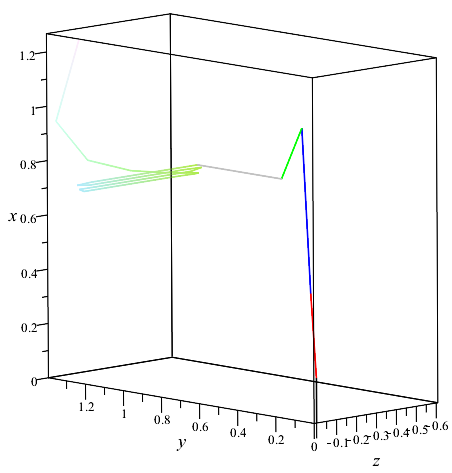
\includegraphics[width=0.50\textwidth]{figs/t1_anima3D_base_rig}
 	\caption{Simulação no ambiente 3D para a Tarefa 1}
 	\label{fig::t1_anima3D_base_rig}
\end{figure}

Estes resultados representam uma referência para posterior comparação com os
resultados obtidos para o modelo MBS acoplado.

\subsubsection{Posição da ferramenta}

Os resultados de simulação da posição da ponta da ferramenta para Tarefa 1 são
apresentados a seguir. A Figura~\ref{fig::t1_posf_base_rig} fornece o valor de
cada coordenada $x, y, z$ no referencial inercial (linha cheia) e também o valor
de referência (linha tracejada), fornecido pela cinemática inversa. A
Figura~\ref{fig::t1_erroposf_base_rig} fornece o erro de posição, ou seja, a
diferença entre o valor de referência dado pela cinemática inversa e o efetivo,
de cada coordenada, assim como o erro absoluto (linha tracejada).

\begin{figure}[h!]
	\centering 
 	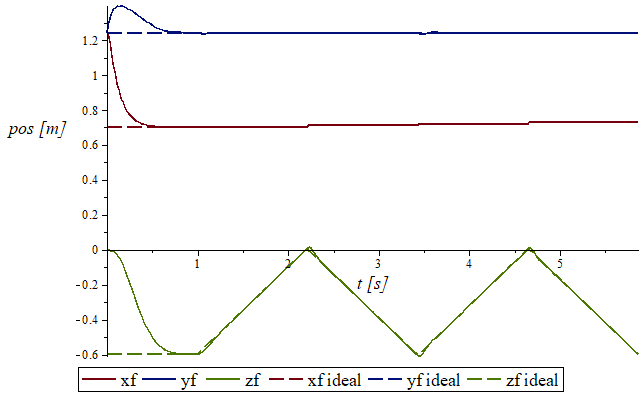
\includegraphics[width=0.80\textwidth]{figs/t1_posf_base_rig}
 	\caption{Posições das coordenadas da ferramenta para base rígida -- Tarefa 1}
 	\label{fig::t1_posf_base_rig}
\end{figure}

\begin{figure}[h!]
	\centering 
 	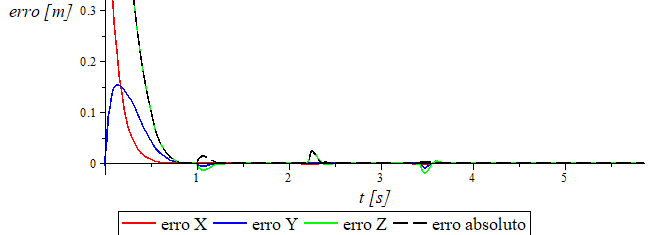
\includegraphics[width=0.80\textwidth]{figs/t1_erroposf_base_rig}
 	\caption{Erro de posição da ferramenta para base rígida -- Tarefa 1}
 	\label{fig::t1_erroposf_base_rig}
\end{figure}


\subsubsection{Trajetória da ferramenta}

A Figura~\ref{fig::t1_traj_base_rig} apresenta a trajetória da ferramenta
projetada no plano $xz$ (linha cheia) e a trajetória de referência (linha
tracejada).
Note-se que os eixos não estão na mesma escala, para facilitar a visualização da
trajetória.

\begin{figure}[h!]
	\centering 
 	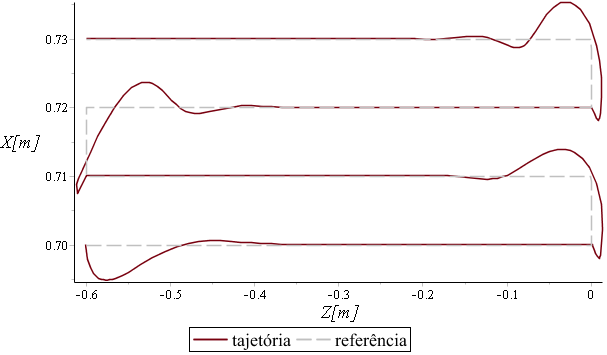
\includegraphics[width=0.80\textwidth]{figs/t1_traj_base_rig}
 	\caption{Trajetória projetada no plano $zx$ para base rígida -- Tarefa 1}
 	\label{fig::t1_traj_base_rig}
\end{figure}


\subsubsection{Velocidade da ferramenta}

São apresentados os gráficos da velocidade da ponta da ferramenta (linhas
cheias) e as velocidades de referência dadas pela cinemática inversa (linhas
tracejadas), na Figura~\ref{fig::t1_velf_base_rig}. Na
Figura~\ref{fig::t1_errovelf_base_rig} os erros em relação a velocidade de
referência, no referencial inercial.

\begin{figure}[h!]
	\centering 
 	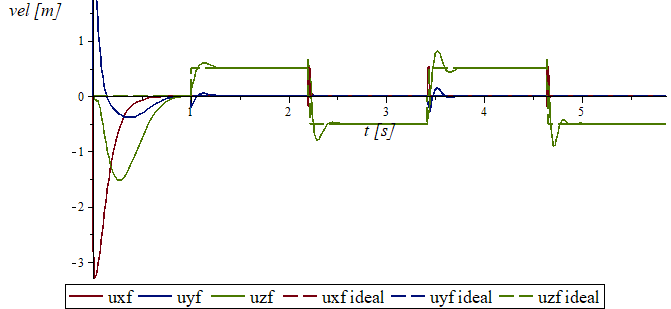
\includegraphics[width=0.80\textwidth]{figs/t1_velf_base_rig}
 	\caption{Velocidades das coordenadas da ferramenta para base rígida -- Tarefa 1}
 	\label{fig::t1_velf_base_rig}
\end{figure}

\begin{figure}[h!]
	\centering 
 	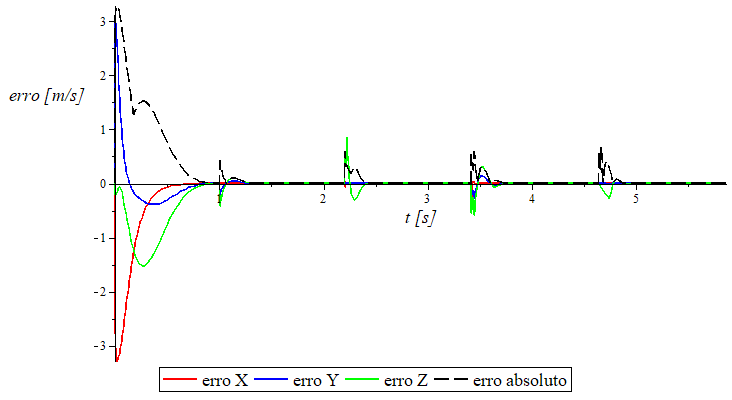
\includegraphics[width=0.80\textwidth]{figs/t1_errovelf_base_rig}
 	\caption{Erro de velocidade da ferramenta para base rígida --
 	Tarefa 1}
 	\label{fig::t1_errovelf_base_rig}
\end{figure}


\subsubsection{Orientação da ferramenta}

O erro de orientação da ferramenta é resultado da matriz de rotação entre o
referencial inercial e a orientação do pulso do robô, em função dos ângulos de
Euler, para a orientação desejada. Faz-se uma transformação da matriz de rotação
em eixo e ângulo, de acordo com as equações~\ref{eq::ang_erro} e
\ref{eq::eixo_erro}. A Figura~\ref{fig::t1_erroori_base_rig} apresenta o
erro de orientação, representado pelo ângulo $\theta$, para a Tarefa 1.

\begin{figure}[h!]
	\centering 
 	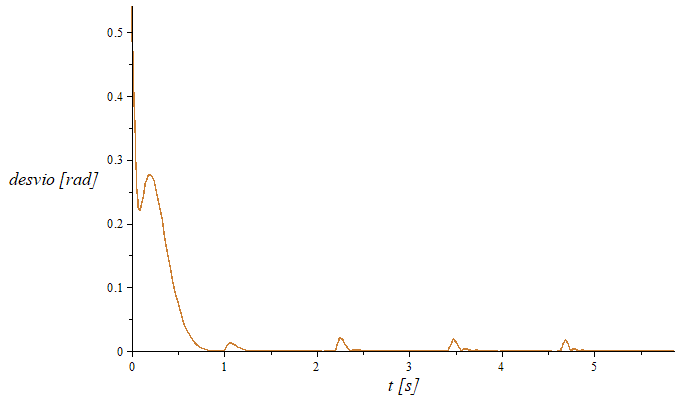
\includegraphics[width=0.80\textwidth]{figs/t1_erroori_base_rig}
 	\caption{Erro de orientação da ferramenta para base rígida -- Tarefa
 	1}
 	\label{fig::t1_erroori_base_rig}
\end{figure}



\subsection{Base de testes -- Tarefa 1} \label{sec::res_testes}

Apresenta-se os resultados das trajetórias considerando o manipulador montado
sobre a base de testes, da seção~\ref{sec::base_testes}, realizando a Tarefa 1.

\subsubsection{Posição do ponto virtual}

O reusltado da Figura~\ref{fig::t1_q123456_base_testes} apresenta a variação das
coordenadas generalizadas $q1$ a $q3$, referentes às translações, e $q4$ a $q6$,
referentes às rotações do ponto virtual de acoplamento base e robô. A
Figura~\ref{fig::t1_pvirtural_base_testes} ilustra o rastro da posição do ponto
virtual (origem do robô) no ambiente 3D.

\begin{figure}[h]
    \centering
    \begin{subfigure}[b]{0.48\textwidth}
        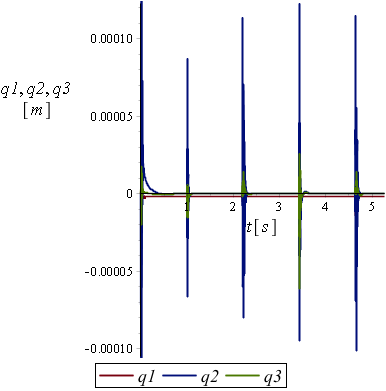
\includegraphics[width=\textwidth]{figs/t1_q123_base_testes}
        \caption{Deslocamentos do ponto virtual}
        \label{fig::t1_q123_base_testes}
    \end{subfigure}
    \quad %add desired spacing between images, e. g. ~, \quad, \qquad, \hfill
    % etc.
      %(or a blank line to force the subfigure onto a new line)
    \begin{subfigure}[b]{0.48\textwidth}
        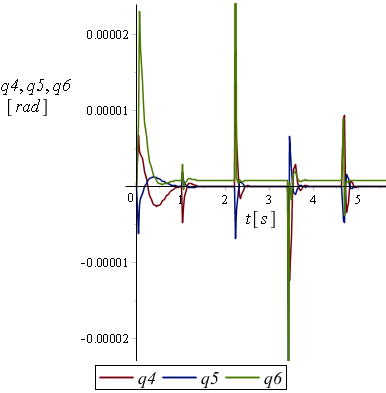
\includegraphics[width=\textwidth]{figs/t1_q456_base_testes}
        \caption{Rotações do ponto virtual}
        \label{fig::t1_q456_base_testes}
    \end{subfigure}
    \caption{Variações de posição e orientação da base de testes -- Tarefa 1}
    \label{fig::t1_q123456_base_testes}
\end{figure}

\begin{figure}[h!]
	\centering 
 	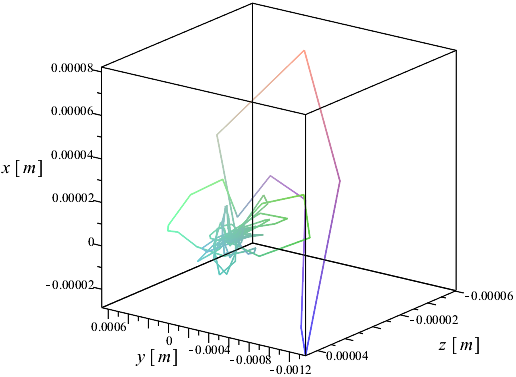
\includegraphics[width=0.70\textwidth]{figs/t1_pvirtural_base_testes}
 	\caption{Rastro da posição do ponto virtual -- Tarefa 1}
 	\label{fig::t1_pvirtural_base_testes}
\end{figure}


\subsubsection{Posição da ferramenta}

A Figura~\ref{fig::t1_posf_base_testes} fornece as posições efetiva (linhas
cheias) e ideal (linhas tracejadas). E a
Figura~\ref{fig::t1_erroposf_base_testes} o erro de cada coordenada, com
respeito ao referencial inercial.

\begin{figure}[h!]
	\centering 
 	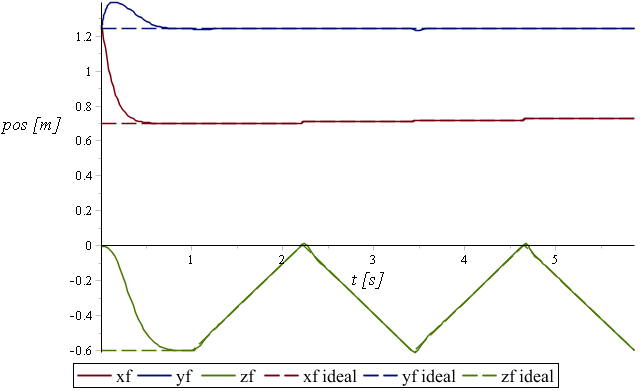
\includegraphics[width=0.80\textwidth]{figs/t1_posf_base_testes}
 	\caption{Posições das coordenadas da ferramenta para base de testes -- Tarefa
 	1}
 	\label{fig::t1_posf_base_testes}
\end{figure}

\begin{figure}[h!]
	\centering 
 	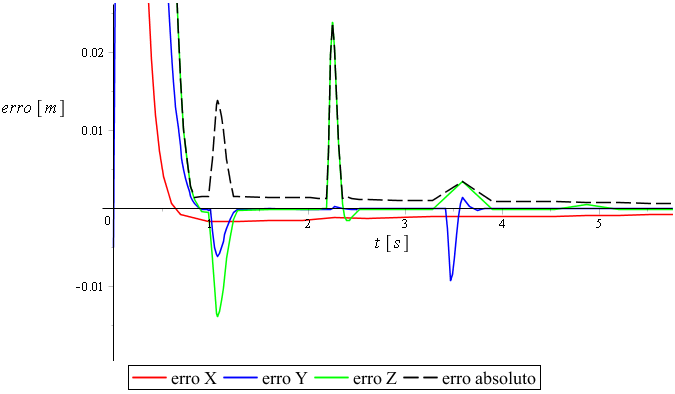
\includegraphics[width=0.80\textwidth]{figs/t1_erroposf_base_testes}
 	\caption{Erro de posição da ferramenta para base de testes -- Tarefa 1}
 	\label{fig::t1_erroposf_base_testes}
\end{figure}


\subsubsection{Trajetória da ferramenta}

A Figura~\ref{fig::t1_traj_base_testes} apresenta a trajetória da ferramenta
projetada no plano $xz$ (linha cheia) e a trajetória de referência (linha
tracejada).
Note-se que os eixos não estão na mesma escala, para facilitar a visualização da
trajetória.

\begin{figure}[h!]
	\centering 
 	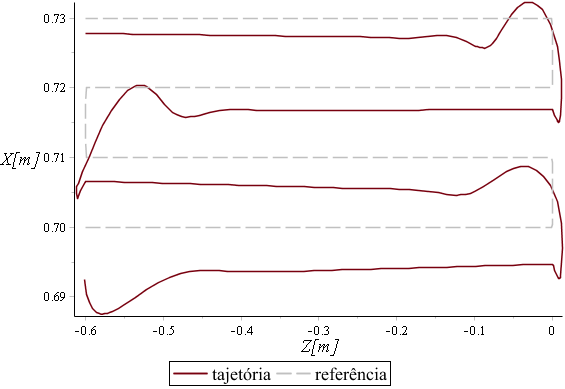
\includegraphics[width=0.70\textwidth]{figs/t1_traj_base_testes}
 	\caption{Trajetória projetada no plano $zx$ para base de testes -- Tarefa 1}
 	\label{fig::t1_traj_base_testes}
\end{figure}


\subsubsection{Velocidade da ferramenta}

São apresentados os gráficos da velocidade da ponta da ferramenta (linhas
cheias) e as velocidades de referência dadas pela cinemática inversa (linhas
tracejadas), na Figura~\ref{fig::t1_velf_base_testes} e na
Figura~\ref{fig::t1_errovelf_base_testes} os erros em relação a velocidade de
referência, no referencial inercial.

\begin{figure}[h!]
	\centering 
 	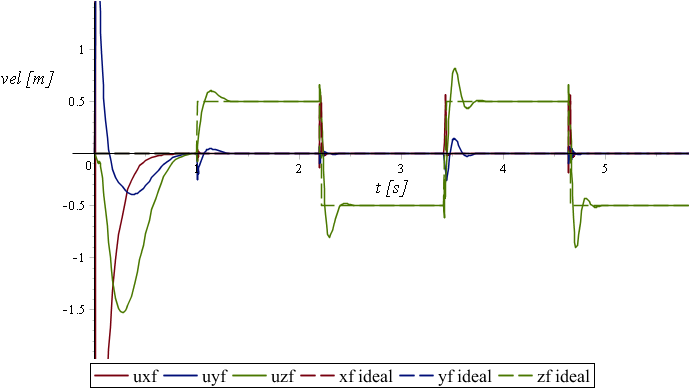
\includegraphics[width=0.80\textwidth]{figs/t1_velf_base_testes}
 	\caption{Velocidades das coordenadas da ferramenta base de testes --
 	Tarefa 1}
 	\label{fig::t1_velf_base_testes}
\end{figure}

\begin{figure}[h!]
	\centering 
 	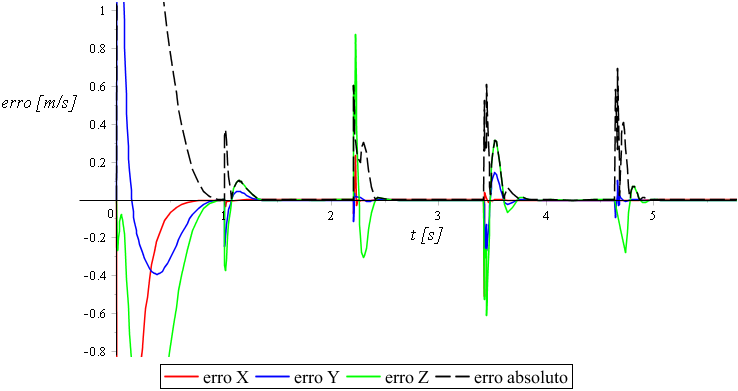
\includegraphics[width=0.80\textwidth]{figs/t1_errovelf_base_testes}
 	\caption{Erro de velocidade da ferramenta para base de testes --
 	Tarefa 1}
 	\label{fig::t1_errovelf_base_testes}
\end{figure}


\subsubsection{Orientação da ferramenta}

A Figura~\ref{fig::t1_erroori_base_testes} apresenta o erro de orientação,
representado pelo ângulo $\theta$.

\begin{figure}[h!]
	\centering 
 	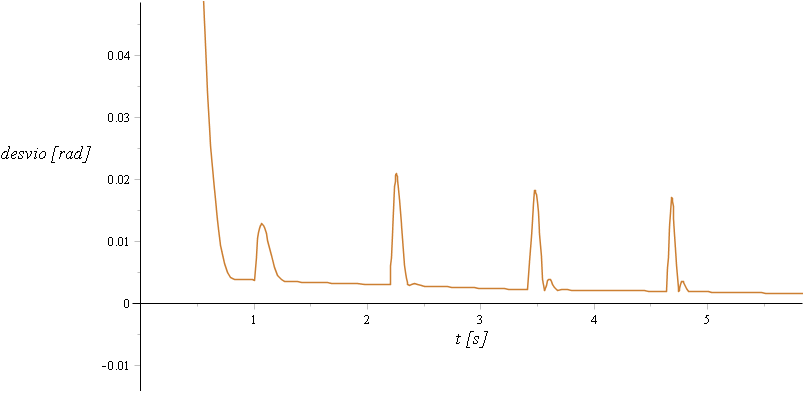
\includegraphics[width=0.80\textwidth]{figs/t1_erroori_base_testes}
 	\caption{Erro de orientação da ferramenta para base de testes -- Tarefa
 	1}
 	\label{fig::t1_erroori_base_testes}
\end{figure}



\subsection{Base modular PRP -- Tarefa 1} \label{sec::res_prp}

Apresenta-se os resultados das trajetórias considerando o manipulador montado
sobre a base modular PRP, da seção~\ref{sec::base_prp}, realizando a Tarefa 1.

\subsubsection{Posição do ponto virtual}

O reusltado da Figura~\ref{fig::t1_q123456_base_prp} apresenta a variação das
coordenadas generalizadas $q1$ a $q3$, referentes às translações, e $q4$ a $q6$,
referentes às rotações do ponto virtual de acoplamento base e robô. A
Figura~\ref{fig::t1_pvirtural_base_prp} ilustra o rastro da posição do ponto
virtual (origem do robô) no ambiente 3D.

\begin{figure}[h]
    \centering
    \begin{subfigure}[b]{0.48\textwidth}
        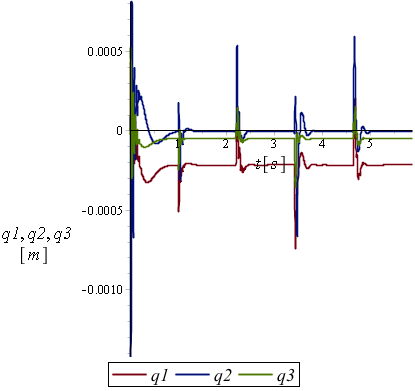
\includegraphics[width=\textwidth]{figs/t1_q123_base_prp}
        \caption{Deslocamentos do ponto virtual}
        \label{fig::t1_q123_base_prp}
    \end{subfigure}
    \quad %add desired spacing between images, e. g. ~, \quad, \qquad, \hfill
    % etc.
      %(or a blank line to force the subfigure onto a new line)
    \begin{subfigure}[b]{0.48\textwidth}
        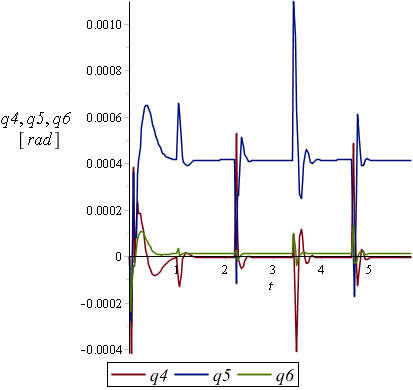
\includegraphics[width=\textwidth]{figs/t1_q456_base_prp}
        \caption{Rotações do ponto virtual}
        \label{fig::t1_q456_base_prp}
    \end{subfigure}
    \caption{Variações de posição e orientação da base PRP -- Tarefa 1}
    \label{fig::t1_q123456_base_prp}
\end{figure}

\begin{figure}[h!]
	\centering 
 	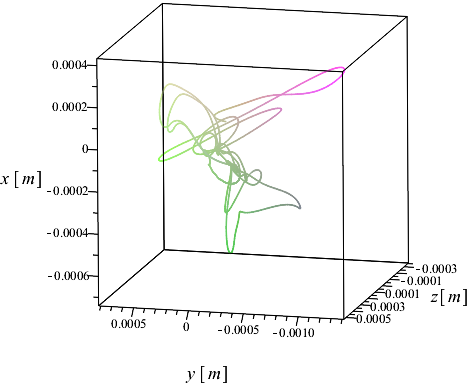
\includegraphics[width=0.70\textwidth]{figs/t1_pvirtural_base_prp}
 	\caption{Rastro da posição do ponto virtual -- Tarefa 1}
 	\label{fig::t1_pvirtural_base_prp}
\end{figure}


\subsubsection{Posição da ferramenta}

A Figura~\ref{fig::t1_posf_base_prp} fornece as posições efetiva (linhas cheias)
e ideal (linhas tracejadas). E a Figura~\ref{fig::t1_erroposf_base_prp} o erro
de cada coordenada, com respeito ao referencial inercial.

\begin{figure}[h!]
	\centering 
 	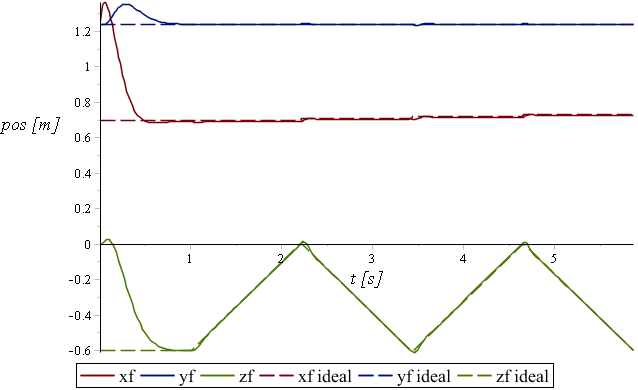
\includegraphics[width=0.80\textwidth]{figs/t1_posf_base_prp}
 	\caption{Posições das coordenadas da ferramenta para base PRP -- Tarefa
 	1}
 	\label{fig::t1_posf_base_prp}
\end{figure}

\begin{figure}[h!]
	\centering 
 	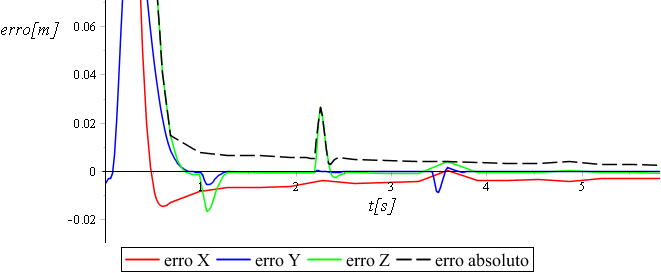
\includegraphics[width=0.80\textwidth]{figs/t1_erroposf_base_prp}
 	\caption{Erro de posição da ferramenta para base PRP -- Tarefa 1}
 	\label{fig::t1_erroposf_base_prp}
\end{figure}


\subsubsection{Trajetória da ferramenta}

A Figura~\ref{fig::t1_traj_base_prp} apresenta a trajetória da ferramenta
projetada no plano $xz$ (linha cheia) e a trajetória de referência (linha
tracejada).
Note-se que os eixos não estão na mesma escala, para facilitar a visualização da
trajetória.

\begin{figure}[h!]
	\centering 
 	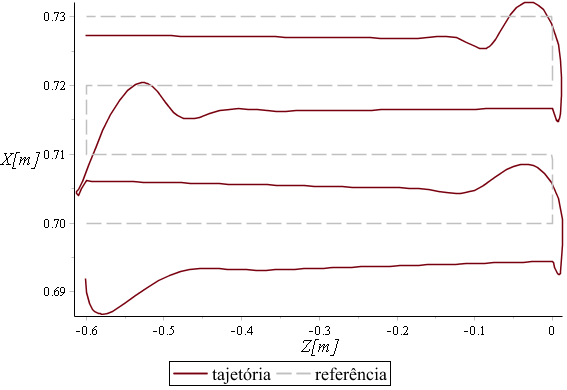
\includegraphics[width=0.70\textwidth]{figs/t1_traj_base_prp}
 	\caption{Trajetória projetada no plano para base PRP -- Tarefa 1}
 	\label{fig::t1_traj_base_prp}
\end{figure}


\subsubsection{Velocidade da ferramenta}

São apresentados os gráficos da velocidade da ponta da ferramenta (linhas
cheias) e as velocidades de referência dadas pela cinemática inversa (linhas
tracejadas), na Figura~\ref{fig::t1_velf_base_prp} e na
Figura~\ref{fig::t1_errovelf_base_prp} os erros em relação a velocidade de
referência, no referencial inercial.

\begin{figure}[h!]
	\centering 
 	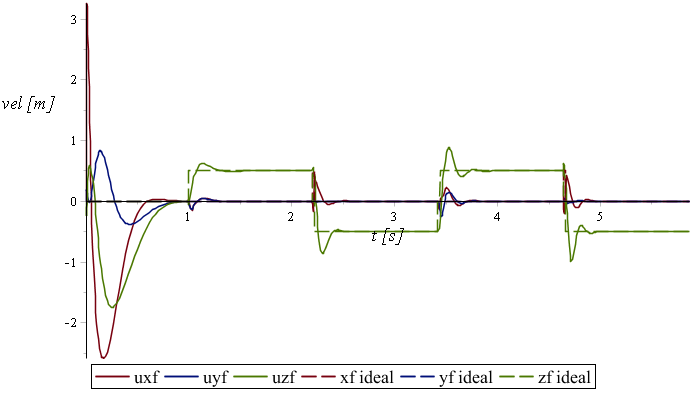
\includegraphics[width=0.80\textwidth]{figs/t1_velf_base_prp}
 	\caption{Velocidades das coordenadas da ferramenta base PRP --
 	Tarefa 1}
 	\label{fig::t1_velf_base_prp}
\end{figure}

\begin{figure}[h!]
	\centering 
 	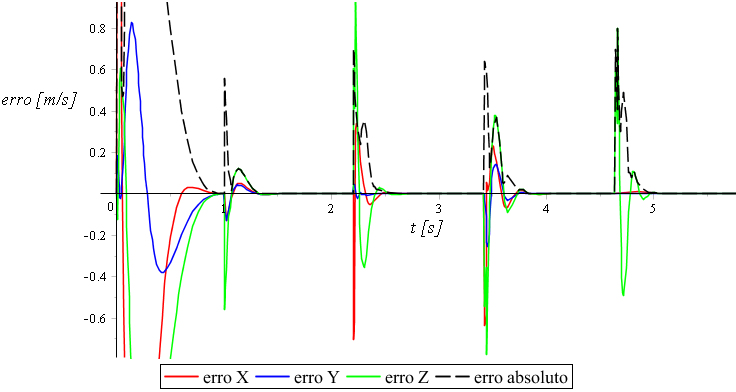
\includegraphics[width=0.80\textwidth]{figs/t1_errovelf_base_prp}
 	\caption{Erro de velocidade da ferramenta para base PRP --
 	Tarefa 1}
 	\label{fig::t1_errovelf_base_prp}
\end{figure}


\subsubsection{Orientação da ferramenta}

A Figura~\ref{fig::t1_erroori_base_prp} apresenta o erro de orientação,
representado pelo ângulo $\theta$.

\begin{figure}[h!]
	\centering 
 	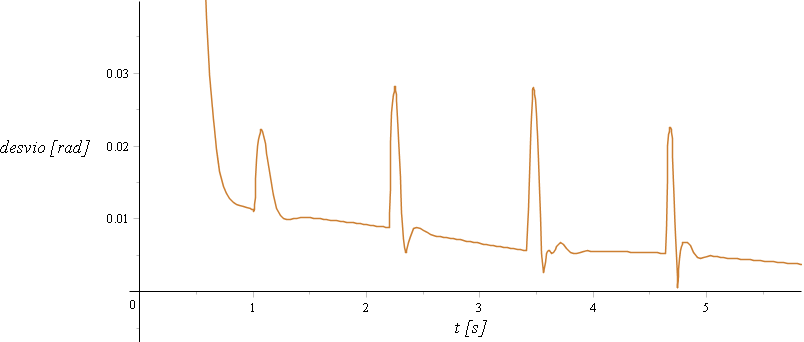
\includegraphics[width=0.80\textwidth]{figs/t1_erroori_base_prp}
 	\caption{Erro de orientação da ferramenta para base PRP -- Tarefa
 	1}
 	\label{fig::t1_erroori_base_prp}
\end{figure}



\subsection{Base telescópica PRPP -- Tarefa 1} \label{sec::res_prpp}

\subsubsection{Posição do ponto virtual}

\subsubsection{Posição da ferramenta}

\subsubsection{Trajetória da ferramenta}

\subsubsection{Velocidade da ferramenta}

\subsubsection{Orientação da ferramenta}


\newpage
% -.~.-.~.-.~.-.~.-.~.-.~.-.~.-.~.-.~ TAREFA 2 ~.-.~.-.~.-.~.-.~.-.~.-.~.
\section{Resultados de simulação da Tarefa 2} \label{sec::resultados_t2}

\subsection{Base rígida -- Tarefa 2}

Seguem os resultados do modelo de base rígida que utiliza o modelo MBS --
Robô.
A Figura~\ref{fig::t2_anima3D_base_rig} apresenta o resultado da simulação no ambiente
3D para a Tarefa 2.

\begin{figure}[h!]
	\centering 
 	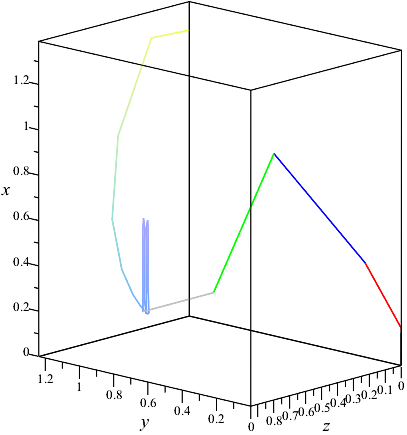
\includegraphics[width=0.50\textwidth]{figs/t2_anima3D_base_rig}
 	\caption{Simulação no ambiente 3D para a Tarefa 2}
 	\label{fig::t2_anima3D_base_rig}
\end{figure}


\subsubsection{Posição da ferramenta}

A Figura~\ref{fig::t2_posf_base_rig} fornece as posições efetiva (linhas cheias)
e ideal (linhas tracejadas). 

\begin{figure}[h!]
	\centering 
 	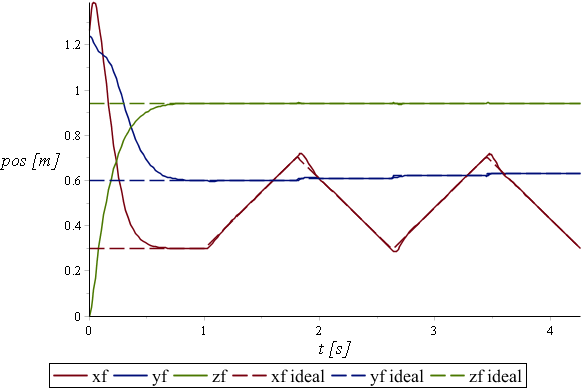
\includegraphics[width=0.80\textwidth]{figs/t2_posf_base_rig}
 	\caption{Posições das coordenadas da ferramenta para base rígida -- Tarefa 2}
 	\label{fig::t2_posf_base_rig}
\end{figure}

E a Figura~\ref{fig::t2_erroposf_base_rig} o erro
de cada coordenada, com respeito ao referencial inercial.

\begin{figure}[h]
	\centering 
 	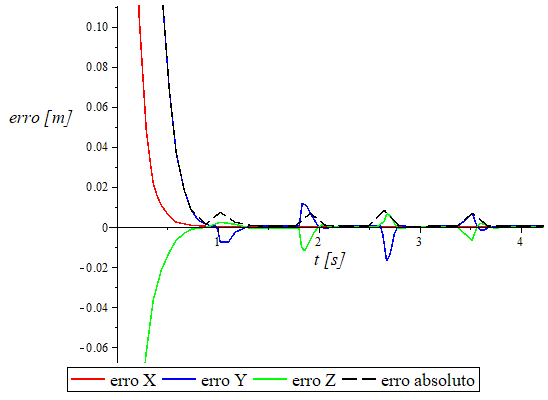
\includegraphics[width=0.70\textwidth]{figs/t2_erroposf_base_rig}
 	\caption{Erro de posição da ferramenta para base rígida -- Tarefa 2}
 	\label{fig::t2_erroposf_base_rig}
\end{figure}


\subsubsection{Trajetória da ferramenta}

A Figura~\ref{fig::t2_traj_base_rig} apresenta a trajetória da ferramenta
projetada no plano $xy$ (linha cheia) e a trajetória de referência (linha
tracejada).

\begin{figure}[h]
	\centering 
 	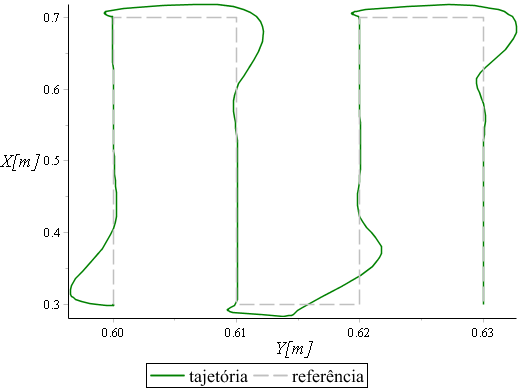
\includegraphics[width=0.70\textwidth]{figs/t2_traj_base_rig}
 	\caption{Trajetória projetada no plano $yx$ para base rígida -- Tarefa 2}
 	\label{fig::t2_traj_base_rig}
\end{figure}


\subsubsection{Velocidade da ferramenta}

São apresentados os gráficos da velocidade da ponta da ferramenta (linhas
cheias) e as velocidades de referência dadas pela cinemática inversa (linhas
tracejadas), na Figura~\ref{fig::t2_velf_base_rig} e na
Figura~\ref{fig::t2_errovelf_base_rig} os erros em relação a velocidade de
referência, no referencial inercial.

\begin{figure}[h]
	\centering 
 	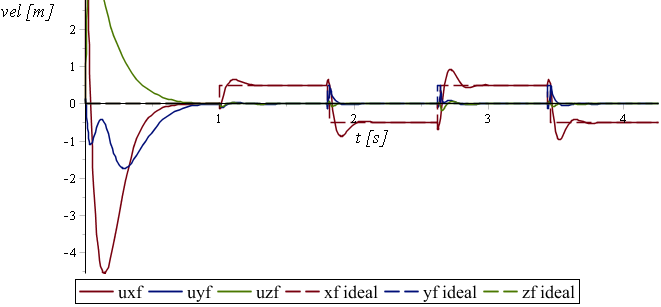
\includegraphics[width=0.85\textwidth]{figs/t2_velf_base_rig}
 	\caption{Velocidades das coordenadas da ferramenta base rígida -- Tarefa
 	2}
 	\label{fig::t2_velf_base_rig}
\end{figure}

\begin{figure}[h]
	\centering 
 	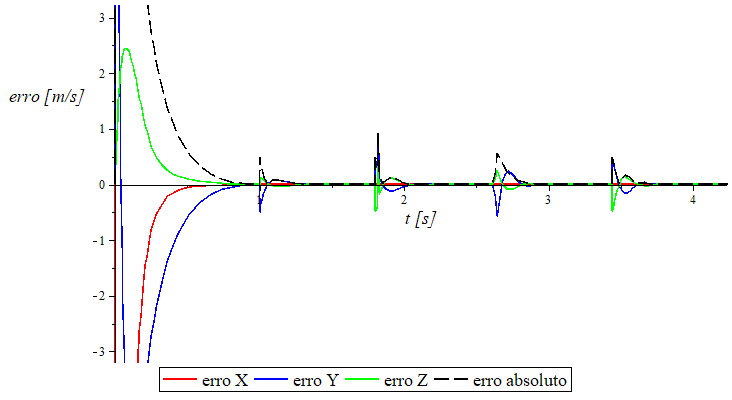
\includegraphics[width=0.85\textwidth]{figs/t2_errovelf_base_rig}
 	\caption{Erro de velocidade da ferramenta para base rígida -- Tarefa 2}
 	\label{fig::t2_errovelf_base_rig}
\end{figure}


\subsubsection{Orientação da ferramenta}

A Figura~\ref{fig::t2_erroori_base_rig} apresenta o erro de orientação da
ferramenta, representado pelo ângulo $\theta$.

\begin{figure}[h]
	\centering 
 	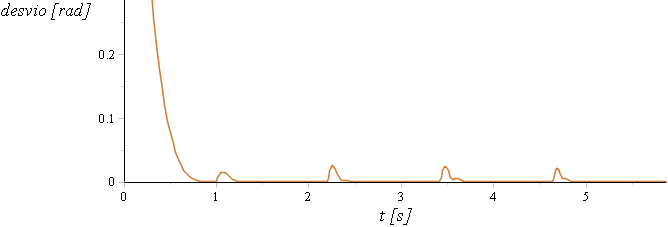
\includegraphics[width=0.80\textwidth]{figs/t2_erroori_base_rig}
 	\caption{Erro de orientação da ferramenta para base rígida -- Tarefa
 	2}
 	\label{fig::t2_erroori_base_rig}
\end{figure}


\subsection{Base de testes -- Tarefa 2}

\subsubsection{Posição do ponto virtual}

O reusltado da Figura~\ref{fig::t2_q123456_base_testes} apresenta a variação das
coordenadas generalizadas $q1$ a $q3$, referentes às translações, e $q4$ a $q6$,
referentes às rotações do ponto virtual de acoplamento base e robô. A
Figura~\ref{fig::t2_pvirtural_base_testes} ilustra o rastro da posição do ponto
virtual (origem do robô) no ambiente 3D.

\begin{figure}[h]
    \centering
    \begin{subfigure}[b]{0.48\textwidth}
        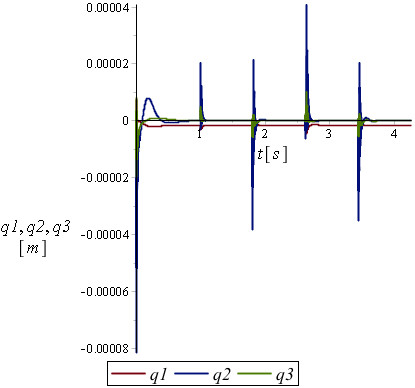
\includegraphics[width=\textwidth]{figs/t2_q123_base_testes}
        \caption{Deslocamentos do ponto virtual}
        \label{fig::t2_q123_base_testes}
    \end{subfigure}
    \quad %add desired spacing between images, e. g. ~, \quad, \qquad, \hfill
    % etc.
      %(or a blank line to force the subfigure onto a new line)
    \begin{subfigure}[b]{0.48\textwidth}
        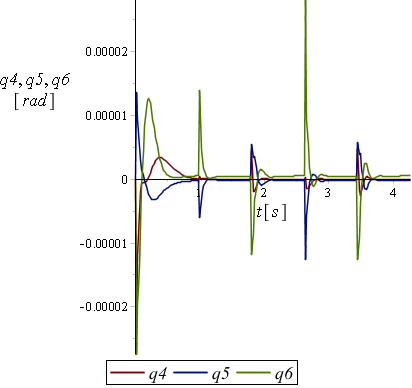
\includegraphics[width=\textwidth]{figs/t2_q456_base_testes}
        \caption{Rotações do ponto virtual}
        \label{fig::t2_q456_base_testes}
    \end{subfigure}
    \caption{Variações de posição e orientação da base de testes -- Tarefa 2}
    \label{fig::t2_q123456_base_testes}
\end{figure}

\begin{figure}[h!]
	\centering 
 	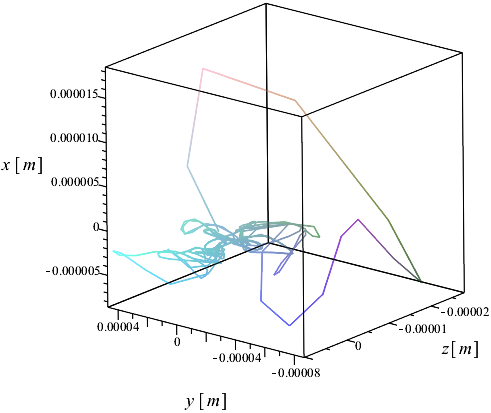
\includegraphics[width=0.60\textwidth]{figs/t2_pvirtural_base_testes}
 	\caption{Rastro da posição do ponto virtual -- Tarefa 2}
 	\label{fig::t2_pvirtural_base_testes}
\end{figure}


\subsubsection{Posição da ferramenta}

A Figura~\ref{fig::t2_posf_base_testes} fornece as posições efetiva e ideal da
Tarefa 2, e a Figura~\ref{fig::t2_erroposf_base_testes} o erro de cada
coordenada, com respeito ao referencial inercial.

\begin{figure}[h!]
	\centering 
 	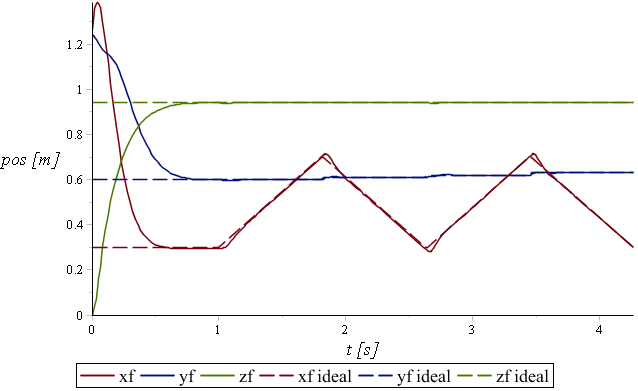
\includegraphics[width=0.75\textwidth]{figs/t2_posf_base_testes}
 	\caption{Posições das coordenadas da ferramenta para base de testes -- Tarefa
 	2}
 	\label{fig::t2_posf_base_testes}
\end{figure}

\begin{figure}[h!]
	\centering 
 	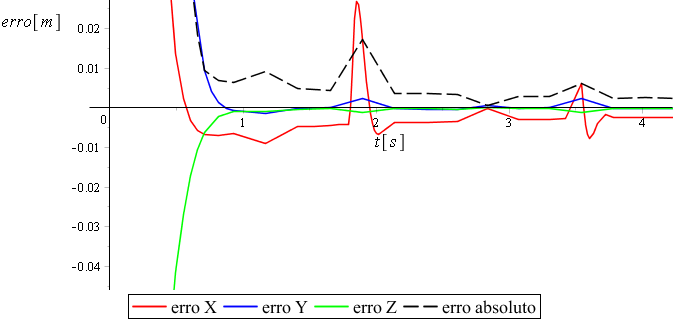
\includegraphics[width=0.75\textwidth]{figs/t2_erroposf_base_testes}
 	\caption{Erro de posição da ferramenta para base de testes -- Tarefa 2}
 	\label{fig::t2_erroposf_base_testes}
\end{figure}


\subsubsection{Trajetória da ferramenta}

A Figura~\ref{fig::t2_traj_base_testes} apresenta a trajetória da ferramenta
projetada no plano $xy$ (linha cheia) e a trajetória de referência (linha
tracejada).

\begin{figure}[h!]
	\centering 
 	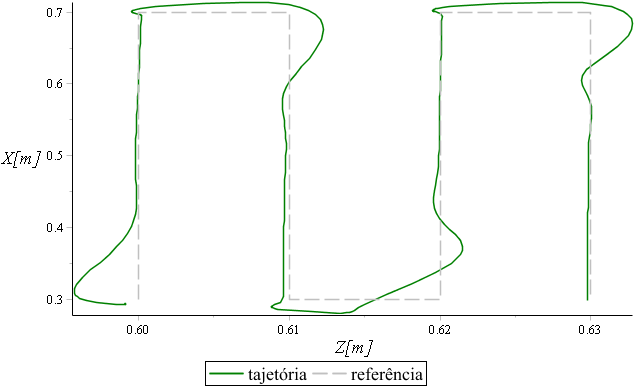
\includegraphics[width=0.70\textwidth]{figs/t2_traj_base_testes}
 	\caption{Trajetória projetada no plano para base de testes -- Tarefa 2}
 	\label{fig::t2_traj_base_testes}
\end{figure}


\subsubsection{Velocidade da ferramenta}

A Figura~\ref{fig::t2_posf_base_testes} fornece as velocidades
efetivas e ideais . A Figura~\ref{fig::t2_erroposf_base_testes} o erro de cada
coordenada, com respeito ao referencial inercial.

\begin{figure}[h!]
	\centering 
 	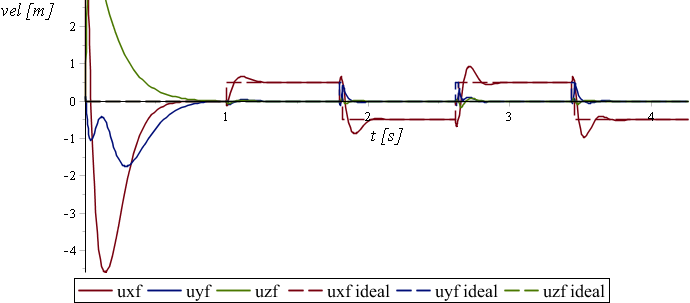
\includegraphics[width=0.80\textwidth]{figs/t2_velf_base_testes}
 	\caption{Velocidades das coordenadas da ferramenta base de testes --
 	Tarefa 2}
 	\label{fig::t2_velf_base_testes}
\end{figure}

\begin{figure}[h!]
	\centering 
 	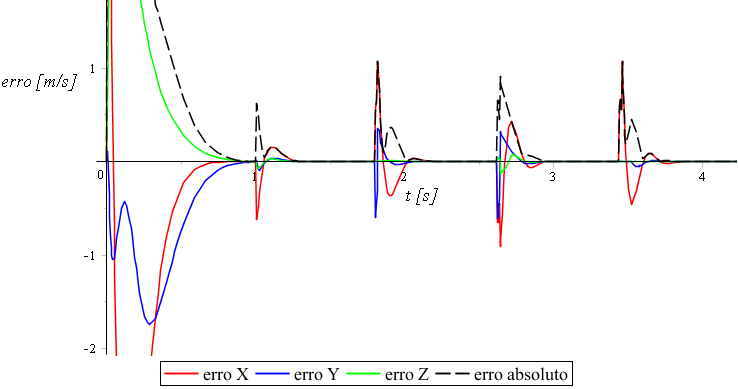
\includegraphics[width=0.80\textwidth]{figs/t2_errovelf_base_testes}
 	\caption{Erro de velocidade da ferramenta para base de testes --
 	Tarefa 2}
 	\label{fig::t2_errovelf_base_testes}
\end{figure}


\subsubsection{Orientação da ferramenta}

A Figura~\ref{fig::t2_erroori_base_testes} apresenta o erro de orientação da
ferramenta, representado pelo ângulo $\theta$.

\begin{figure}[h!]
	\centering 
 	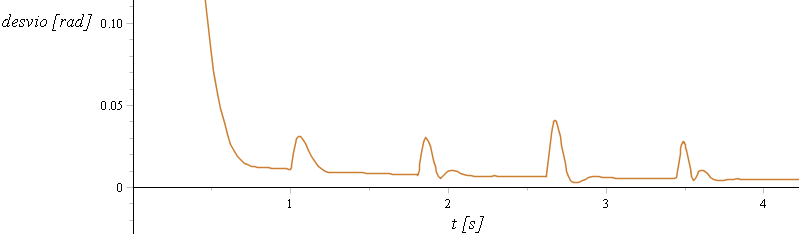
\includegraphics[width=0.80\textwidth]{figs/t2_erroori_base_testes}
 	\caption{Erro de orientação da ferramenta para base de testes -- Tarefa
 	2}
 	\label{fig::t2_erroori_base_testes}
\end{figure}



\subsection{Base PRP -- Tarefa 2}

\subsubsection{Posição do ponto virtual}

O reusltado da Figura~\ref{fig::t2_q123456_base_prp} apresenta a variação das
coordenadas generalizadas $q1$ a $q3$, referentes às translações, e $q4$ a $q6$,
referentes às rotações do ponto virtual de acoplamento base e robô. A
Figura~\ref{fig::t2_pvirtural_base_prp} ilustra o rastro da posição do ponto
virtual (origem do robô) no ambiente 3D.

\begin{figure}[h]
    \centering
    \begin{subfigure}[b]{0.48\textwidth}
        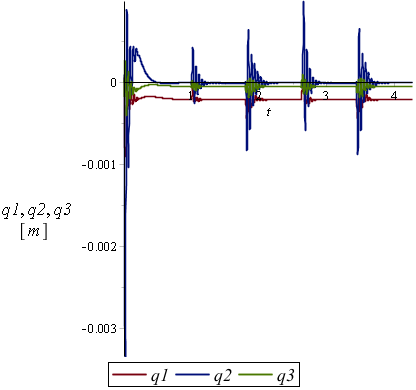
\includegraphics[width=\textwidth]{figs/t2_q123_base_prp}
        \caption{Deslocamentos do ponto virtual}
        \label{fig::t2_q123_base_prp}
    \end{subfigure}
    \quad %add desired spacing between images, e. g. ~, \quad, \qquad, \hfill
    % etc.
      %(or a blank line to force the subfigure onto a new line)
    \begin{subfigure}[b]{0.48\textwidth}
        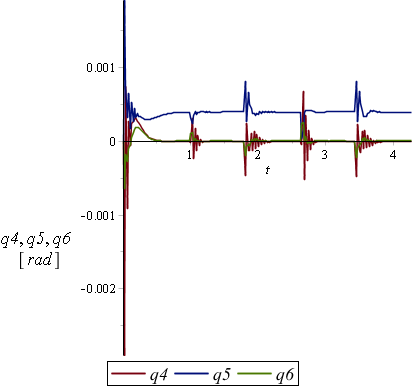
\includegraphics[width=\textwidth]{figs/t2_q456_base_prp}
        \caption{Rotações do ponto virtual}
        \label{fig::t2_q456_base_prp}
    \end{subfigure}
    \caption{Variações de posição e orientação da base PRP -- Tarefa 2}
    \label{fig::t2_q123456_base_prp}
\end{figure}

\begin{figure}[h!]
	\centering 
 	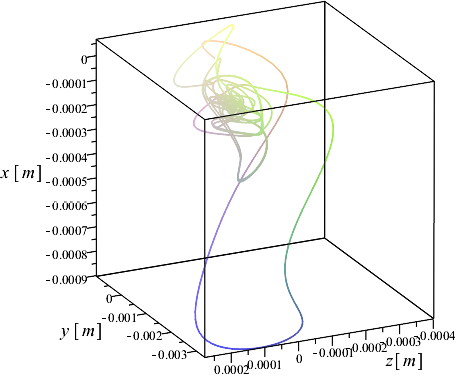
\includegraphics[width=0.70\textwidth]{figs/t2_pvirtural_base_prp}
 	\caption{Rastro da posição do ponto virtual -- Tarefa 2}
 	\label{fig::t2_pvirtural_base_prp}
\end{figure}


\subsubsection{Posição da ferramenta}

A Figura~\ref{fig::t2_posf_base_prp} fornece as posições efetiva e ideal da
Tarefa 2, e a Figura~\ref{fig::t2_erroposf_base_prp} o erro de cada
coordenada, com respeito ao referencial inercial.

\begin{figure}[h!]
	\centering 
 	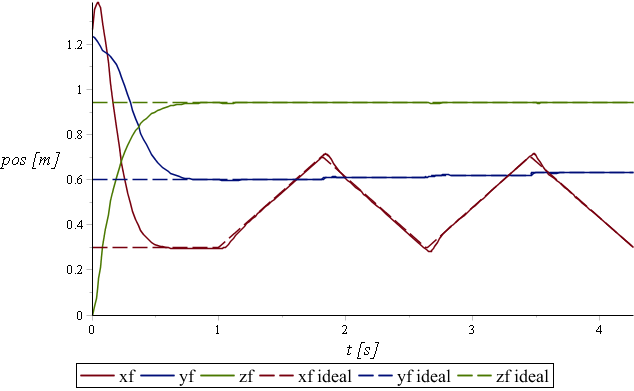
\includegraphics[width=0.80\textwidth]{figs/t2_posf_base_prp}
 	\caption{Posições das coordenadas da ferramenta para base PRP -- Tarefa
 	2}
 	\label{fig::t2_posf_base_prp}
\end{figure}

\begin{figure}[h!]
	\centering 
 	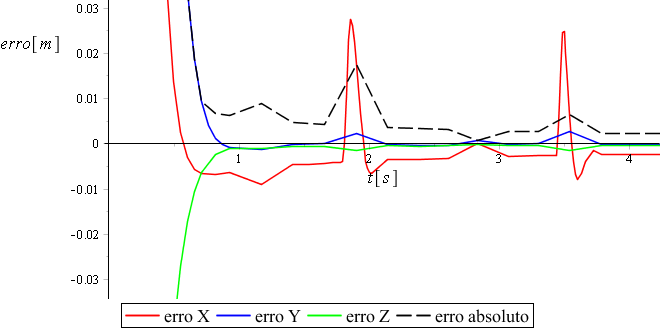
\includegraphics[width=0.80\textwidth]{figs/t2_erroposf_base_prp}
 	\caption{Erro de posição da ferramenta para base PRP -- Tarefa 2}
 	\label{fig::t2_erroposf_base_prp}
\end{figure}


\subsubsection{Trajetória da ferramenta}

A Figura~\ref{fig::t2_traj_base_prp} apresenta a trajetória da ferramenta
projetada no plano $xy$ (linha cheia) e a trajetória de referência (linha
tracejada).

\begin{figure}[h!]
	\centering 
 	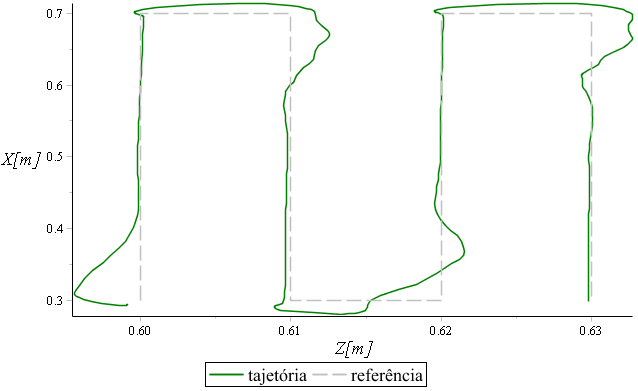
\includegraphics[width=0.80\textwidth]{figs/t2_traj_base_prp}
 	\caption{Trajetória projetada no plano para base PRP -- Tarefa 2}
 	\label{fig::t2_traj_base_prp}
\end{figure}


\subsubsection{Velocidade da ferramenta}

A Figura~\ref{fig::t2_posf_base_prp} fornece as velocidades
efetivas e ideais . A Figura~\ref{fig::t2_erroposf_base_prp} o erro de cada
coordenada, com respeito ao referencial inercial.

\begin{figure}[h!]
	\centering 
 	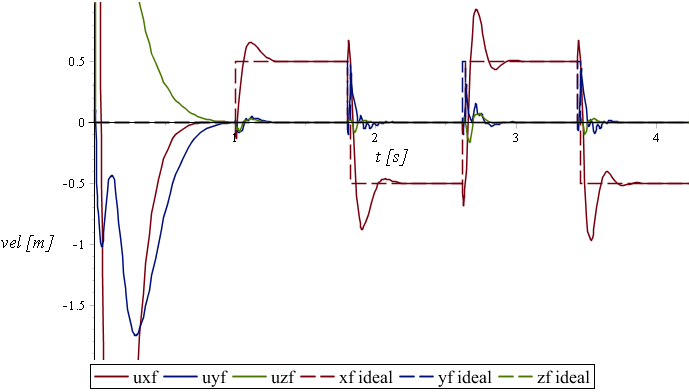
\includegraphics[width=0.80\textwidth]{figs/t2_velf_base_prp}
 	\caption{Velocidades das coordenadas da ferramenta base PRP --
 	Tarefa 2}
 	\label{fig::t2_velf_base_prp}
\end{figure}

\begin{figure}[h!]
	\centering 
 	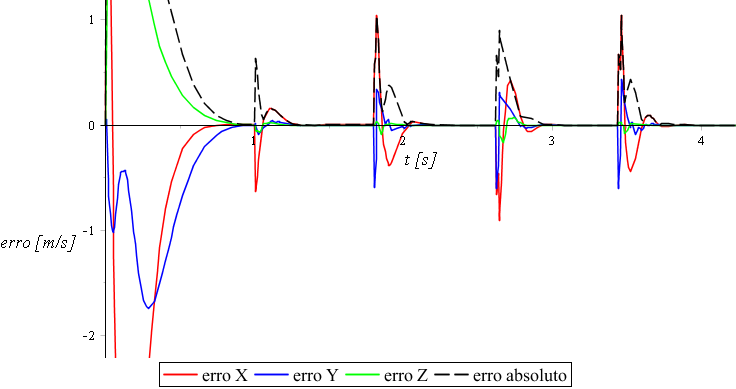
\includegraphics[width=0.80\textwidth]{figs/t2_errovelf_base_prp}
 	\caption{Erro de velocidade da ferramenta para base PRP --
 	Tarefa 2}
 	\label{fig::t2_errovelf_base_prp}
\end{figure}


\subsubsection{Orientação da ferramenta}

A Figura~\ref{fig::t2_erroori_base_prp} apresenta o erro de orientação da
ferramenta, representado pelo ângulo $\theta$.

\begin{figure}[h!]
	\centering 
 	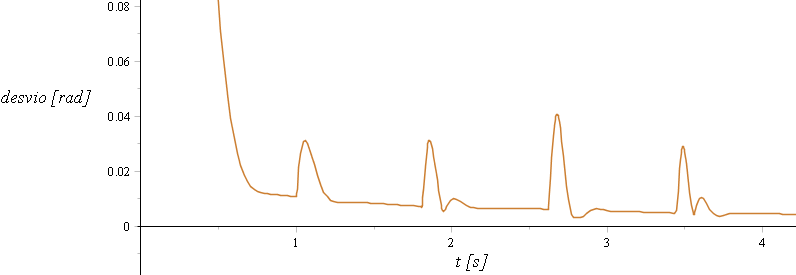
\includegraphics[width=0.80\textwidth]{figs/t2_erroori_base_prp}
 	\caption{Erro de orientação da ferramenta para base PRP -- Tarefa
 	2}
 	\label{fig::t2_erroori_base_prp}
\end{figure}



\subsection{Base PRPP -- Tarefa 2}

\subsubsection{Posição do ponto virtual}

\subsubsection{Posição da ferramenta}

\subsubsection{Trajetória da ferramenta}

\subsubsection{Velocidade da ferramenta}

\subsubsection{Orientação da ferramenta}

% -.~.-.~.-.~.-.~.-.~.-.~.-.~.-.~.-.~.-.~.-.~.-
\section{Comparação dos resultados} \label{sec::comparacao}

\subsection{Erros máximos}

As Tabelas~\ref{tab::erros_base_rig} a \ref{tab::erros_base_prpp} resumem os
erros máximos de posição, velocidade e orientação encontrados em cada tarefa. Os
erros de posição são dados nas 3 coordenadas cartesianas do referencial
inercial; o erro de velocidade é fornecido na direção tangente da trajetória; e
o erro de orientação é dado como um ângulo $\theta$ na direção do eixo $\omega$.

\subsubsection{Base rígida}

\begin{table}[h!]
\centering
\caption{Resumo dos erros máximos encontrados -- Base Rígida}
\label{tab::erros_base_rig}
\begin{tabular}{@{}ccccccc@{}}
\toprule
         & \multicolumn{3}{c}{\textbf{Posição $[mm]$}} & \textbf{Velocidade $[m/s]$} & \multicolumn{2}{c}{\textbf{Orientação $[rad]$}} 	\\ \midrule
         & x          & y          & z          & tangente            & $\theta$            & $\omega$         		\\
Tarefa 1 & 1,5        & 9,0        & 20,0       & 0,30                &	0,021				& [0,995,~-0,960,~-0,029]                  	\\
Tarefa 2 & 0,07       & 16,5	   & 11,5       & 0,45                & 0,032				& [0,999,~0,002,~0,046] \\ \bottomrule
\end{tabular}
\end{table}


\subsubsection{Base de testes}

\begin{table}[h!]
\centering
\caption{Resumo dos erros máximos encontrados -- Base de testes}
\label{tab::erros_base_testes}
\begin{tabular}{@{}ccccccc@{}}
\toprule
         & \multicolumn{3}{c}{\textbf{Posição $[mm]$}} & \textbf{Velocidade $[m/s]$} & \multicolumn{2}{c}{\textbf{Orientação $[rad]$}} 	\\ \midrule
         & x          & y          & z          & tangente            & $\theta$            & $\omega$         		\\
Tarefa 1 & 1,5    	  & 9,1        & 13,3       & 0,9                 &	0,021				& [0.989,~-0,098,~0,111]                  	\\
Tarefa 2 & 26     	  & 2,2 	   & 1,1        & 0,9                 & 0,041				& [-0,130,~-0.830,~0,557] \\ \bottomrule
\end{tabular}
\end{table}


\subsubsection{Base PRP}

\begin{table}[h!]
\centering
\caption{Resumo dos erros máximos encontrados -- Base PRP}
\label{tab::erros_base_prp}
\begin{tabular}{@{}ccccccc@{}}
\toprule
         & \multicolumn{3}{c}{\textbf{Posição $[mm]$}} & \textbf{Velocidade $[m/s]$} & \multicolumn{2}{c}{\textbf{Orientação $[rad]$}} 	\\ \midrule
         & x          & y			& z			& tangente		& $\theta$		& $\omega$		\\
Tarefa 1 &     	 	  &				&			&				&				& [,~,~]		\\
Tarefa 2 &      	  &				&			&				&				& [,~,~]		\\ \bottomrule
\end{tabular}
\end{table}


% -.~.-.~.-.~.-.~.-.~.-.~.-.~.-.~.-.~.-.~.-.~.-
\section{Possíveis soluções} \label{sec::solucoes}

% if we have a proper knowledge about the dynamics of the system including the
% base motion dynamics, we can develop sophisticated control methods.
% (Artigo: Moving base robotics and reaction management control)
